% Preamble
% Note that in this TeX file we use for each new sentence a new line. 
% Doing so allows us to better track changes and updates via Git.20210901
% 
\documentclass[10pt]{article}
% Packages
\usepackage[left=0.8in, right=0.8in, top=0.8in, bottom=1in]{geometry} % set the margins to 'narrow'
\setlength\parindent{0pt} % remove the indent before the first line in paragraph
\setlength{\parskip}{\baselineskip} % add space between paragraphs
\usepackage{amsmath}
\usepackage{longtable} % break long tables
\usepackage{pdflscape}  % rotate pages by 90 degrees
\usepackage{rotating} % rotate tables, etc. by 90 degrees
\usepackage{booktabs} % to typeset your table
\usepackage{graphicx} % to include pdf as figures
\usepackage{subfig} % to allow for subplots within one figure
\usepackage{longtable} % for long tables across several pages
\usepackage{float} % to prevent table position moving use H in e.g., \begin{figure}[H]
\restylefloat{table} % to prevent table position moving
\usepackage{hyperref} % to enable preview and links on references
\usepackage[table]{xcolor} % to enable colors in tables
\hypersetup{
	colorlinks=false,
	linkcolor=black,
	citecolor=black,
	filecolor=black,
	urlcolor=black,  
} 
\usepackage{amssymb,amsmath,amsfonts}
\usepackage{array} % for new columns types
% define new column types to align column and specify the width
\usepackage{lineno}
\linenumbers
\newcolumntype{L}[1]{>{\raggedright\let\newline\\\arraybackslash\hspace{0pt}}m{#1}}
\newcolumntype{C}[1]{>{\centering\let\newline\\\arraybackslash\hspace{0pt}}m{#1}}
\newcolumntype{R}[1]{>{\raggedleft\let\newline\\\arraybackslash\hspace{0pt}}m{#1}}
\usepackage{lastpage} % for total page numbers
\usepackage{fancyhdr} % for header and footer - page numbers
\pagestyle{fancy} % for header and footer - page numbers
\rfoot{}
\renewcommand{\headrulewidth}{0pt} % remove the top vertical line of {fancyhdr}
\rhead{}
% set input path to plots and table folders:
\newcommand*{\InputsFolderPath}{C:/DEV/DML/src/data/}
\newcommand*{\InputsPath}{\InputsFolderPath/20221110/}
%
\title{Double/Debiased Machine Learning comparison study}
% Document
\begin{document}
\maketitle
\abstract{TBA}
\section{Motivation}
Double/Debiased machine learning model is especially suited for the analysis of causal effects.

The following analysis bases on the Python package "DoubleML" from \cite{Bach2022}. 
In the following, we will use the implementation and the data generation processes (DGP) for different variations of the Double/Debiased Machine Learning approach and compare their performance.
All scripts for the analysis in this github repository: \url{https://github.com/g-r-m-n/dml}.

\section{Double/Debiased Machine Learning Model}
\subsection{Partial linear regression model}
We want to analyze the relationship of an $(n \times 1 )$ outcome variable $Y$ and a $(n \times 1 )$ treatment or policy variable $D$. 
There is a $(n \times k )$ matrix $X$ of $k$ $(n \times 1 )$ variables $x_l$, $l=1,...,k$ which are related to $Y$ but are not of primary interest.
These variables are related to the treatment $D$ and are therefore denoted as confunding or control variables.
We assume the following partially linear regression (PLR) model for the relationship of $Y$, $D$ and $X$ \cite{Cher2018}.
\begin{eqnarray}\label{dml_plr_1}
Y &=& D \theta_0 + g_0(X) + U, \;\;\; E[U|X,D] =0  	\\ \label{dml_plr_2}
D &=&  m_0(X) + V, \;\;\; E[V|X] =0  	
\end{eqnarray}
$g_0$ and $m_0$ are function of mapping $X$ to $\mathbb{R}$. 
$g_0$ and $m_0$ are also denoted as nuisance functions because their specific functional forms are not of central interest.
$U$ and $V$ are $(n \times 1 )$ vectors of error terms or disturbances. 
$\theta_0$ is scalar parameter that measures the effect of $D$ on $Y$ and is of central interest.\footnote{
Note that we assume that the treatment $D$ is additive linear related to $Y$. 
Doing so helps for an easily understandable description of the approach.
We will relax the assumption of linear additivity in next subsection below.}
$ E[V|X]$ denotes the expected value of the variable $V$ given the variables $X$.
	
Note that we cannot estimate $g_0$ from Equation \eqref{dml_plr_1} alone. 
The reason is that not only $g_0$ is a function of $X$ but also $D$ is via \eqref{dml_plr_2}. 
Denote the approach where we estimate $g_0$ from Equation \eqref{dml_plr_1} alone as naive approach.
The in the naive approach, we would for example iterate until convergence between updating $g_0$ using $Y - D \theta_0 = g_0(X) + U$ and updating $\theta_0$ using $Y - g_0(X) = D \theta_0 + U$. 
An estimate of $g_0$ from the naive approach would be biased as it does not account for the fact that $Y - D \theta_0$ is depended of $X$, i.e., $ m_0(X) = E[X|D] $.
However $ g_0(X) \ne E[Y|X] $ because $Y$ depends also on $D \theta_0$.

\cite{Cher2018} propose an algorithm to estimate the treatment effect parameter $\theta_0$ from the PLR model from above unbiased and $n^{-1/2}$ root consistent using machine learning (ML) to assess $g_0$ and $m_0$ if the ML estimators are at least  $n^{-1/4}$ root consistent.  
This is where the name Double/Debiased ML (DML) comes from. 
The algorithm uses cross fitting and the idea of partialing-out to avoid the regularization bias.  
We outline the latter in more detail below. 
\begin{enumerate}
	\item Estimate $D =  \hat{m}_0(X) + \hat{V}$. This is the treatment model where we now partial out the effect of $X$ from $D$.
	\item Estimate $Y = D  \hat{\theta}_0 +  \hat{g}_0(X) +  \hat{U}$ as in the naive approach from above. This is the outcome model where we with $Y - \hat{g}_0(X)$ partial out the effect of $X$ on $Y$ conditional on $D$.
	\item Regress $Y - \hat{g}_0(X)$ on $\hat{V}$ using ordinary least squares (OLS) and denote the resulting parameter as $\check{\theta}_0$.
\end{enumerate}
$\check{\theta}_0$ is treatment effect estimate that is free of regularization bias. 
Note that the partialing-out approach is similar to the residuals-on-residuals regression for linear regression models \cite{frisch1933,Lovell1963,Lovell2008} and for kernel regression models \cite{rob1988}.
We could obtain $\check{\theta}_0$ also if we replaced Step 2. from the partialing-out approach from above with the following $Y = \hat{l}_0(X) + \hat{U} $ and regress in Step 3. $\hat{U}$ on $\hat{V}$ using OLS. 
$l_0$ is a function that maps $X$ to $\mathbb{R}$ reflects $E[Y|X]$.
%In particular, the approach uses moment conditions with Neyman orthogonalitya residuals-on-residuals with 

\subsection{PLR model modifications}
We can extend the PLR model to the following partial linear regression instrumental variables model (PLR-IV). 
\begin{eqnarray*}\label{dml_plr-iv_1}
	Y &=&  D  \theta_0 +  g_0(X) + U, \;\;\; E[U|X,Z] =0  	\\ \label{dml_plr-iv_2}
	Z &=&  m_0(X) + V, \;\;\; E[V|X] =0.
\end{eqnarray*}
$Z$ is $n \times l$ matrix of instrumental variables.
The usage of the instrumental variables allows us to account for the endogeneity of the treatment variables $D$, i.e., that $D$ is (indirectly) correlated with $U$.
%$D$ is endogenous because it is (indirectly) correlated with $U$. 
This is because the error term $U$ is correlated with $V$ and $V$ is correlated with $D$.
%This is $|E(D V)| \ge c$ where $c$ is positive constant, i.e., $c>0$. $E((UV)^2) \ge c^4$.
We can combine Equations \eqref{dml_plr-iv_1} and \eqref{dml_plr-iv_2} to build score function for the inference of $\theta$ and the nuisance functions. 
See \cite{Cher2018} for more details.  %and note that this model specification is equivalent to the one where we model $D$ as a function of $Z$ and $X$ as shown in the Subsection 2.2 below.

The PLR model can be generalized the following interactive regression model (IRM):
\begin{eqnarray*}\label{dml_irm_1}
	Y &=&  g_0(X,D) + U, \;\;\; E[U|X,D] =0  	\\ \label{dml_irm_2}
	D &=&  m_0(X) + V, \;\;\; E[V|X] =0  	.
\end{eqnarray*}
Now the function $g_0$ from Equation \eqref{dml_irm_1} jointly maps $X$ and $D$ to $\mathbb{R}$.
Typically, the treatment variable $D$ is now constrained to be binary, with values 0 and 1.
This way, the average treatment effect (ATE) (and the local average treatment effect, LATE) can be estimated as in \cite{Cher2018}.

The IRM model can be further generalized to an interactive regression model using instrumental variables (IIV) as follows:
\begin{eqnarray*}\label{dml_IIV_1}
	Y &=&  \mu_0(X,Z) + U, \;\;\; E[U|X,Z] =0  	\\ \label{dml_IIV_2}
	D &=&  m_0(X,Z) + V, \;\;\; E[V|X,Z] =0  		\\ \label{dml_IIV_3}
	Z &=&  p_0(X) + \zeta, \;\;\; E[\zeta|X] =0  	.
\end{eqnarray*}
$\mu_0$ is a function that maps $X$ and $Z$ to $\mathbb{R}$.



\section{Simulation experiments}
We conduct in total four simulation experiments, i.e., Scenario 1-4. 
The DGPs increase in terms of complexity for the scenarios and we compare the results from models which are suitable form the underlying data structure.
In each simulation experiment, we create $n=1.000$ observations of data for $k=20$ variables.
We set the treatment effect parameter $\theta$ to 0.5 and replicate the DGP 30 times.
The DGPs of the simulation experiments (A)-(D) are from \cite{Bach2022} and \cite{Bach2021}.\\

Note that we find overall similar performance differences in the comparison of the different approaches in terms of that the double ML models (i.e., PLR, IRM, PLR-IV and IIV) are typically in a similar ballpark as their linear counter parts (i.e., OLS or 2SLS), in case we increase, e.g., the number of observations $n$ or the number of parameters $k$, modify the DGPs and/or hyper-parameter tuning settings.\\


To estimate the non-linear functions in the PLR, IRM, PLR-IV and IIV models, we use random forest models, either classification models if the dependent variable is binary and regression model otherwise.
As hyper-parameters, we sue  100 trees, a maximum of 20 features, a maximum depth of 5 and a minimum sample of 2 per leave.

In addition to the PLR, IRM, PLR-IV and IIV models, we compare the results of the following three models (I)-(III) when suitable.
(I) An linear regression model, denoted as OLS of the following form. 
\begin{eqnarray*}\label{ols}
	Y= D \theta + X \beta + U.
\end{eqnarray*}
(II) A two stage least squares regression model, denoted as 2SLS of the following form. 
\begin{eqnarray*}\label{ols}
	Y &=& D \theta + X \beta sls+ U,\\
	W &=& X \gamma + Z \delta + \zeta + V,
\end{eqnarray*}
where $W$ is a $(n \times (k+1))$ matrix that consists of the matrix $X$ with an additional column which is $D$. 
(III) A naive ML model, denoted as naive-ML of the following form. 
\begin{eqnarray*}\label{ols}
	Y &=& t_0(D, X) + U
\end{eqnarray*}
where $t_0$ is a function that maps D and X to $\mathbb{R}$.



\subsection{Scenario 1}
\subsubsection{DGP: PLR model}
The Scenario 1 represents the case of a PLR model and we use the following DGP for $i=1,...,n$ \cite{Cher2018}.
\begin{eqnarray*}\label{dgp_1.1}
y_i &=& \theta d_i + g_0(x_i) + s_2 \zeta_i, \\
d_i &=& m_0(x_i) + s_1 v_i, \\
x_i &\sim& \mathcal{N}(0, \Sigma),\\
\zeta_i &\sim& \mathcal{N}(0,1),\\
v_i &\sim& \mathcal{N}(0,1),
\end{eqnarray*}
where $d_i, v_i, y_i$ and $\zeta_i$ are the $i^{th}$ entries of $D,V,Y$ and $\zeta$, respectively.
$ \mathcal{N}(\mu_n, \Sigma_n)$ represents the normal distribution with mean value $\mu_n$ and variance $\Sigma_n$.
Note that  $\mu_n$ can be a vector and $\Sigma_n$ is in this case a variance-covariance matrix.
$x_i$ is the $(k \times 1)$ vector of row $i$ from matrix $X$.
$\Sigma$ is a matrix with entries $\sigma_{mj} = 0.7^{|j-m|}$, with $m=1,..,k$ and $j=1,...,k$.
The nuisance functions are given by
\begin{eqnarray*}\label{dgp_1.2}
m_0(x_i) &=& a_0 x_{i,1} + a_1 \frac{\exp(x_{i,3})}{1+\exp(x_{i,3})},\\
g_0(x_i) &=& b_0 \frac{\exp(x_{i,1})}{1+\exp(x_{i,1})} + b_1 x_{i,3}.
\end{eqnarray*}
We use the following parameter values: $a_0=1, a_1=0.25, s_1=1, b_0=1, b_1=0.25$ and $s_2=1$.
Note that the nuisance functions $m_0$ and $g_0$ are non-linear in $x_i$.

\subsubsection{Results}
The Figure \ref{Scenario 1} shows the true and estimated treatment effects per replication for Scenario 1. 
The error bars represent the upper and lower bound of the 95\% confidence interval of the estimate. 
The red line represents the true value of the treatment effect.
\begin{figure}[H]
	\begin{center}
		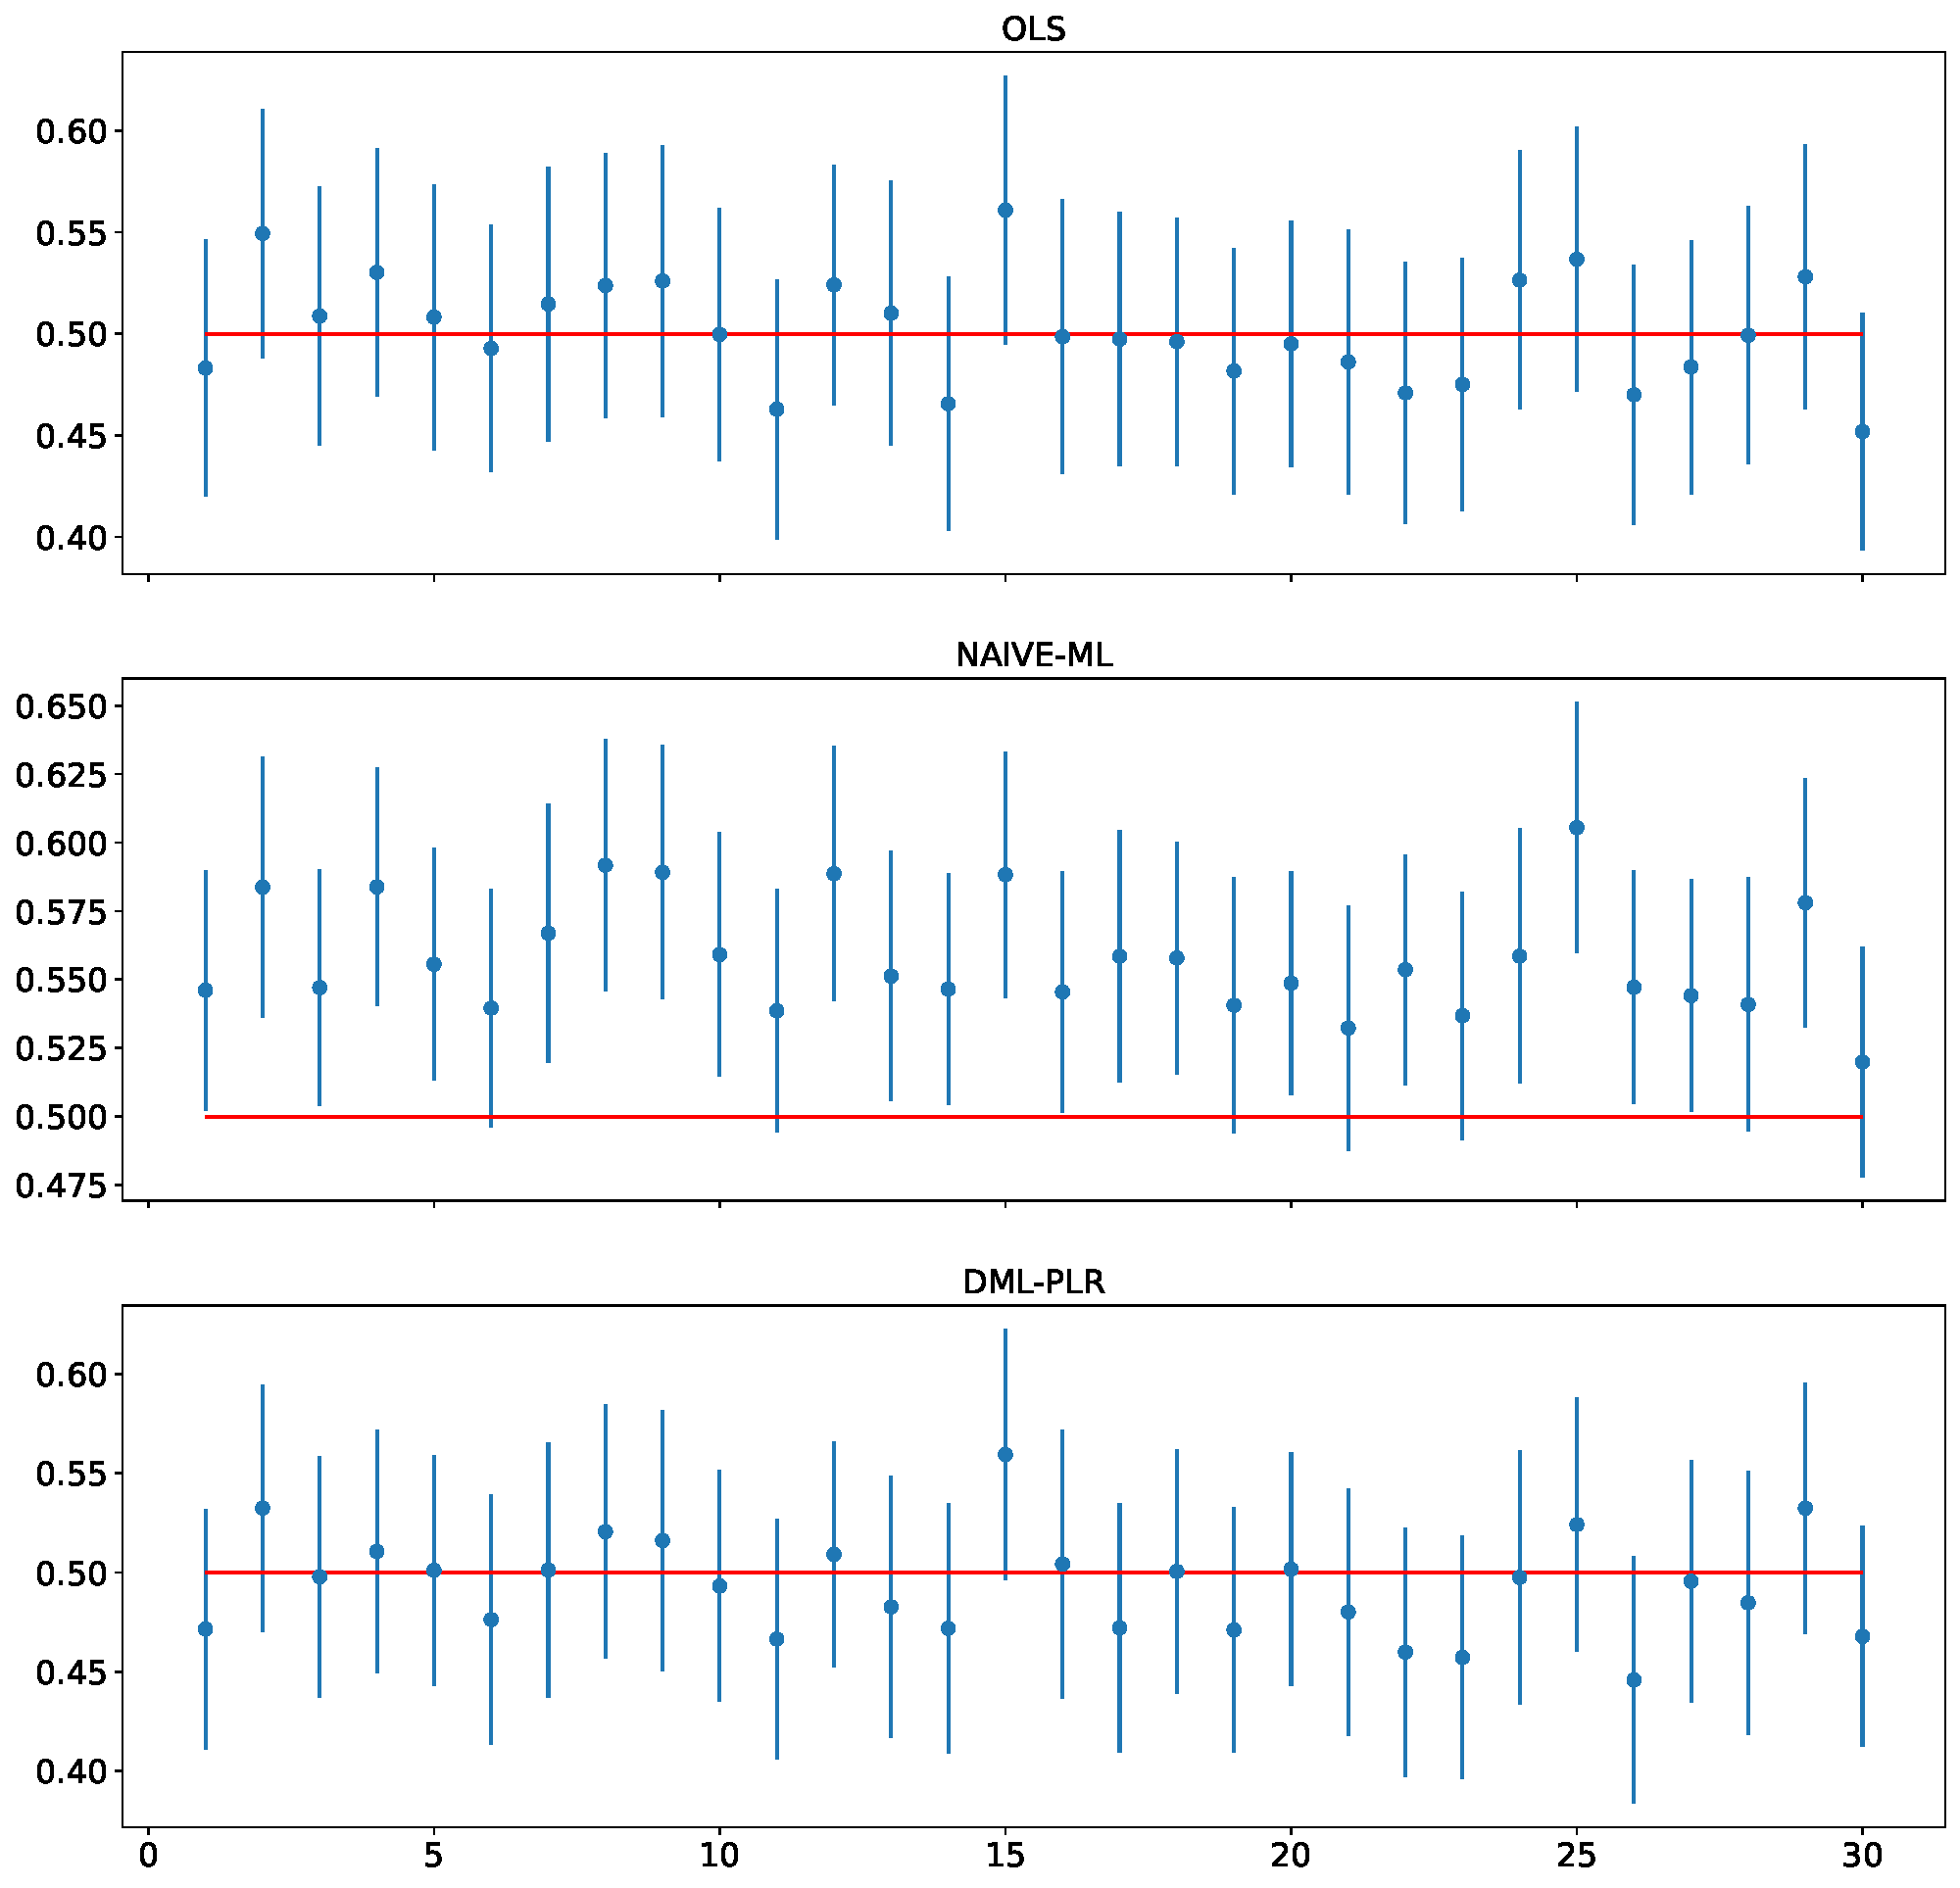
\includegraphics[width=.65\columnwidth]{\InputsPath/plots/Scenario1.pdf}
		\caption{True and estimated treatment effects per replication for Scenario 1. The error bars represent the upper and lower bound of the 95\% confidence interval of the estimate. The red line represents the true value of the treatment effect.}
		\label{Scenario 1}
	\end{center}
\end{figure}
Table \ref{Scenario1} shows the root mean squared error (RMSE), the mean absolute error (MAE) and the bias of estimated treatment effect and the true value across the replications for the compared models.
The last row indicates which model performs best according to RMSE, MAE or bias.
\begin{table}[H]
\centering
\caption{Scenario 1}
\label{Scenario1}
\begin{tabular}{L{3.3333333333333335cm}L{2.6666666666666665cm}R{2.0cm}R{2.6666666666666665cm}}
\toprule
{} &     RMSE &      MAE &    Bias \\
\midrule
OLS      &   0.0267 &   0.0219 & -0.0002 \\
NAIVE-ML &   0.0324 &   0.0267 &  0.0166 \\
DML-PLR  &   0.0247 &   0.0202 & -0.0071 \\
Best     &  DML-PLR &  DML-PLR &     OLS \\
\bottomrule
\end{tabular}
\end{table}

We find in Scenario 1 that the DML-PLR and the OLS model tend to recover the treatment effect overall similarly in terms of how accurate the point estimates are, of how wider the confidence intervals are and in terms of the (absolute) bias.
The NAIVE-ML model performs worse in the RMSE, and MAE and has a larger bias compared to DML-PLR and OLS by a factor of three to four.

\subsection{Scenario 2}
\subsubsection{DGP: IRM model}
The Scenario 2 represents the case of a IRM model and we use the following DGP for $i=1,...,n$.
The data generating process is based on a the simulation experiment in \cite{Bell2017}.
\begin{eqnarray*}\label{dgp_3.1}
	y_i &=& \theta d_i + c_y x_i' \beta d_i + \zeta_i, \\
	d_i &=& 1\left\lbrace \frac{\exp(c_d x_i' \beta)}{1+\exp(c_d x_i' \beta)} > v_i \right\rbrace, \\
	\zeta_i &\sim& \mathcal{N}(0,1), \\	
	v_i
	&\sim& \mathcal{U}(0,1),\\
	x_i &\sim& \mathcal{N}(0, \Sigma),
\end{eqnarray*}
where $\Sigma$ is a matrix with entries $\Sigma_{kj} = 0.5^{|j-m|}$, with $m=1,..,k$ and $j=1,...,k$.
$\mathcal{U}(a,b)$ represents the continuous uniform distribution with parameters $a$ and $b$.
$\beta$ is a $(k\times 1)$ vector with entries $\beta_j=\frac{1}{j^2}$ and the constants $c_y$ and $c_d$ are the following:
\begin{eqnarray*}\label{dgp_3.2}
	c_y = \sqrt{\frac{R_y^2}{(1-R_y^2) \beta' \Sigma \beta}}, \qquad 
	c_d =\sqrt{\frac{(\pi^2 /3) R_d^2}{(1-R_d^2) \beta' \Sigma \beta}}.
\end{eqnarray*}
We set the parameters $R^2_d$ and $R^2_y$ to 0.5.
\subsubsection{Results}
\begin{figure}[H]
	\begin{center}
		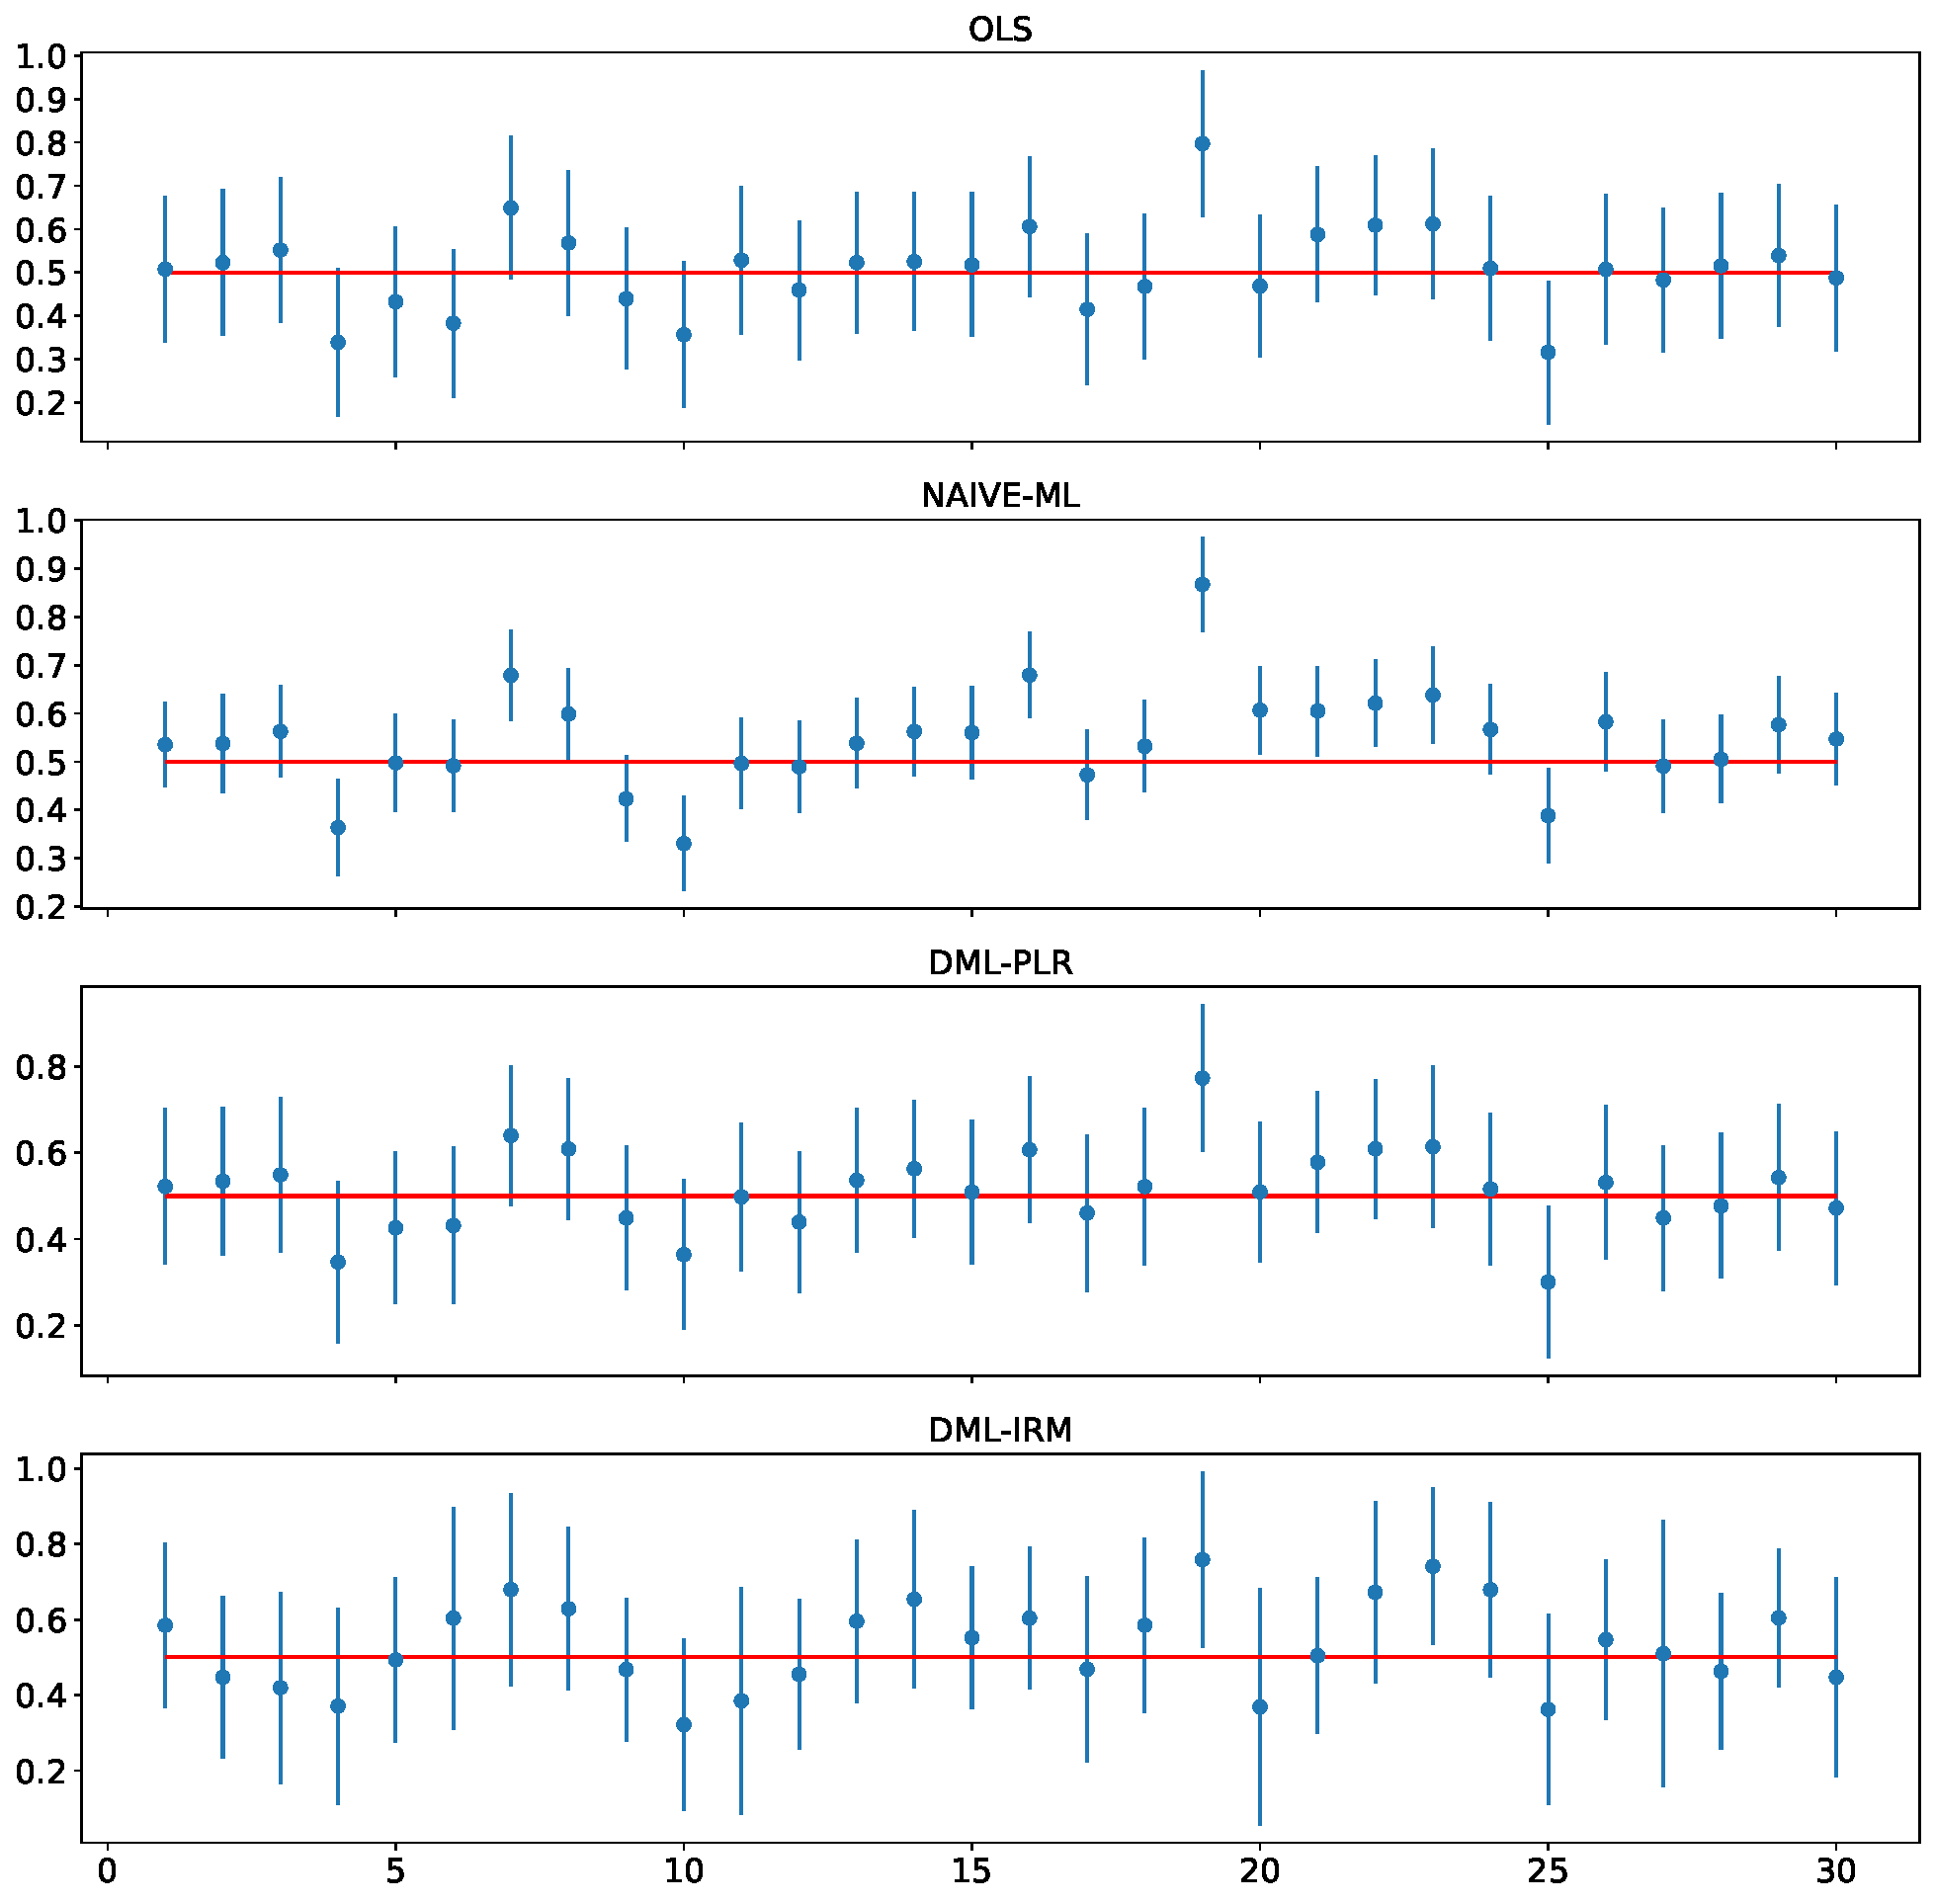
\includegraphics[width=.65\columnwidth]{\InputsPath/plots/Scenario2.pdf}
		\caption{True and estimated treatment effects per replication for Scenario 2. The error bars represent the upper and lower bound of the 95\% confidence interval of the estimate. The red line represents the true value of the treatment effect.}
		\label{Scenario2}
	\end{center}
\end{figure}
\begin{table}[H]
\centering
\caption{Scenario 2}
\label{Scenario2}
\begin{tabular}{L{3.3333333333333335cm}L{2.6666666666666665cm}R{2.0cm}R{2.6666666666666665cm}}
\toprule
{} &     RMSE &      MAE &     Bias \\
\midrule
OLS      &   0.0854 &   0.0699 &  -0.0269 \\
NAIVE-ML &   0.0922 &    0.071 &    0.035 \\
DML-PLR  &   0.0809 &   0.0671 &  -0.0174 \\
DML-IRM  &   0.1306 &   0.1094 &   0.0979 \\
Best     &  DML-PLR &  DML-PLR &  DML-PLR \\
\bottomrule
\end{tabular}
\end{table}

We find in Scenario 2 that the DML-PLR and the OLS model tend to recover the treatment effect overall similarly in terms of how wider the confidence intervals, the RMSE, and MAE. 
DML-IRM and OLS obtain an similar low bias, the one of DML-PLR is slightly higher.
The NAIVE-ML model performs worse across RMSE, MAE and bias.


\subsection{Scenario 3}
\subsubsection{PLR-IV model}
The Scenario 3 represents the case of a PLR-IV model and we use the following DGP for $i=1,...,n$ \cite{Cher2015}.
\begin{eqnarray*}\label{dgp_2.1}
y_i &=& \theta d_i + x_i' \beta + \varepsilon_i,	\\
d_i &=& x_i' \gamma + z_i' \delta + u_i, \\
z_i &=& \Pi x_i + \zeta_i, 
\end{eqnarray*}
with
\begin{eqnarray*}\label{dgp_2.2}
	\left(\begin{matrix} \varepsilon_i \\ u_i \\ \zeta_i \\ x_i \end{matrix} \right) \sim
\mathcal{N}\left(0, \left(\begin{matrix} 1 & 0.6 & 0 & 0 \\ 0.6 & 1 & 0 & 0 \\
	0 & 0 & 0.25 I_{l} & 0 \\ 0 & 0 & 0 & \Sigma \end{matrix} \right) \right)
\end{eqnarray*}
where  $\Sigma$ is a $k \times k$ matrix with entries
$\Sigma_{mj} = 0.5^{|j-m|}$, with $m=1,..,k$ and $j=1,...,k$. 
$I_{l}$ is the $l \times l$ identity matrix.
$\beta = \gamma$ is a $k$-vector with entries $\beta_j=\frac{1}{j^2}$ with  $j=1,...,k$.
$\delta$ is a $l$-vector with entries $\delta_j=\frac{1}{h^2}$, with $h=1,...,l$.
$\Pi$ is a matrix of parameters and specified as follows: $\Pi = (I_{l}, 0_{l \times (k - l)})$, where $ 0_{l \times (k - l)}$ is a $(l \times (k-l))$ matrix of zeros.
Note that the endogeneity of $D$ comes from the non-zero correlation of $\varepsilon_i$ and $u_i$.
\subsubsection{Results}
\begin{figure}[H]
	\begin{center}
		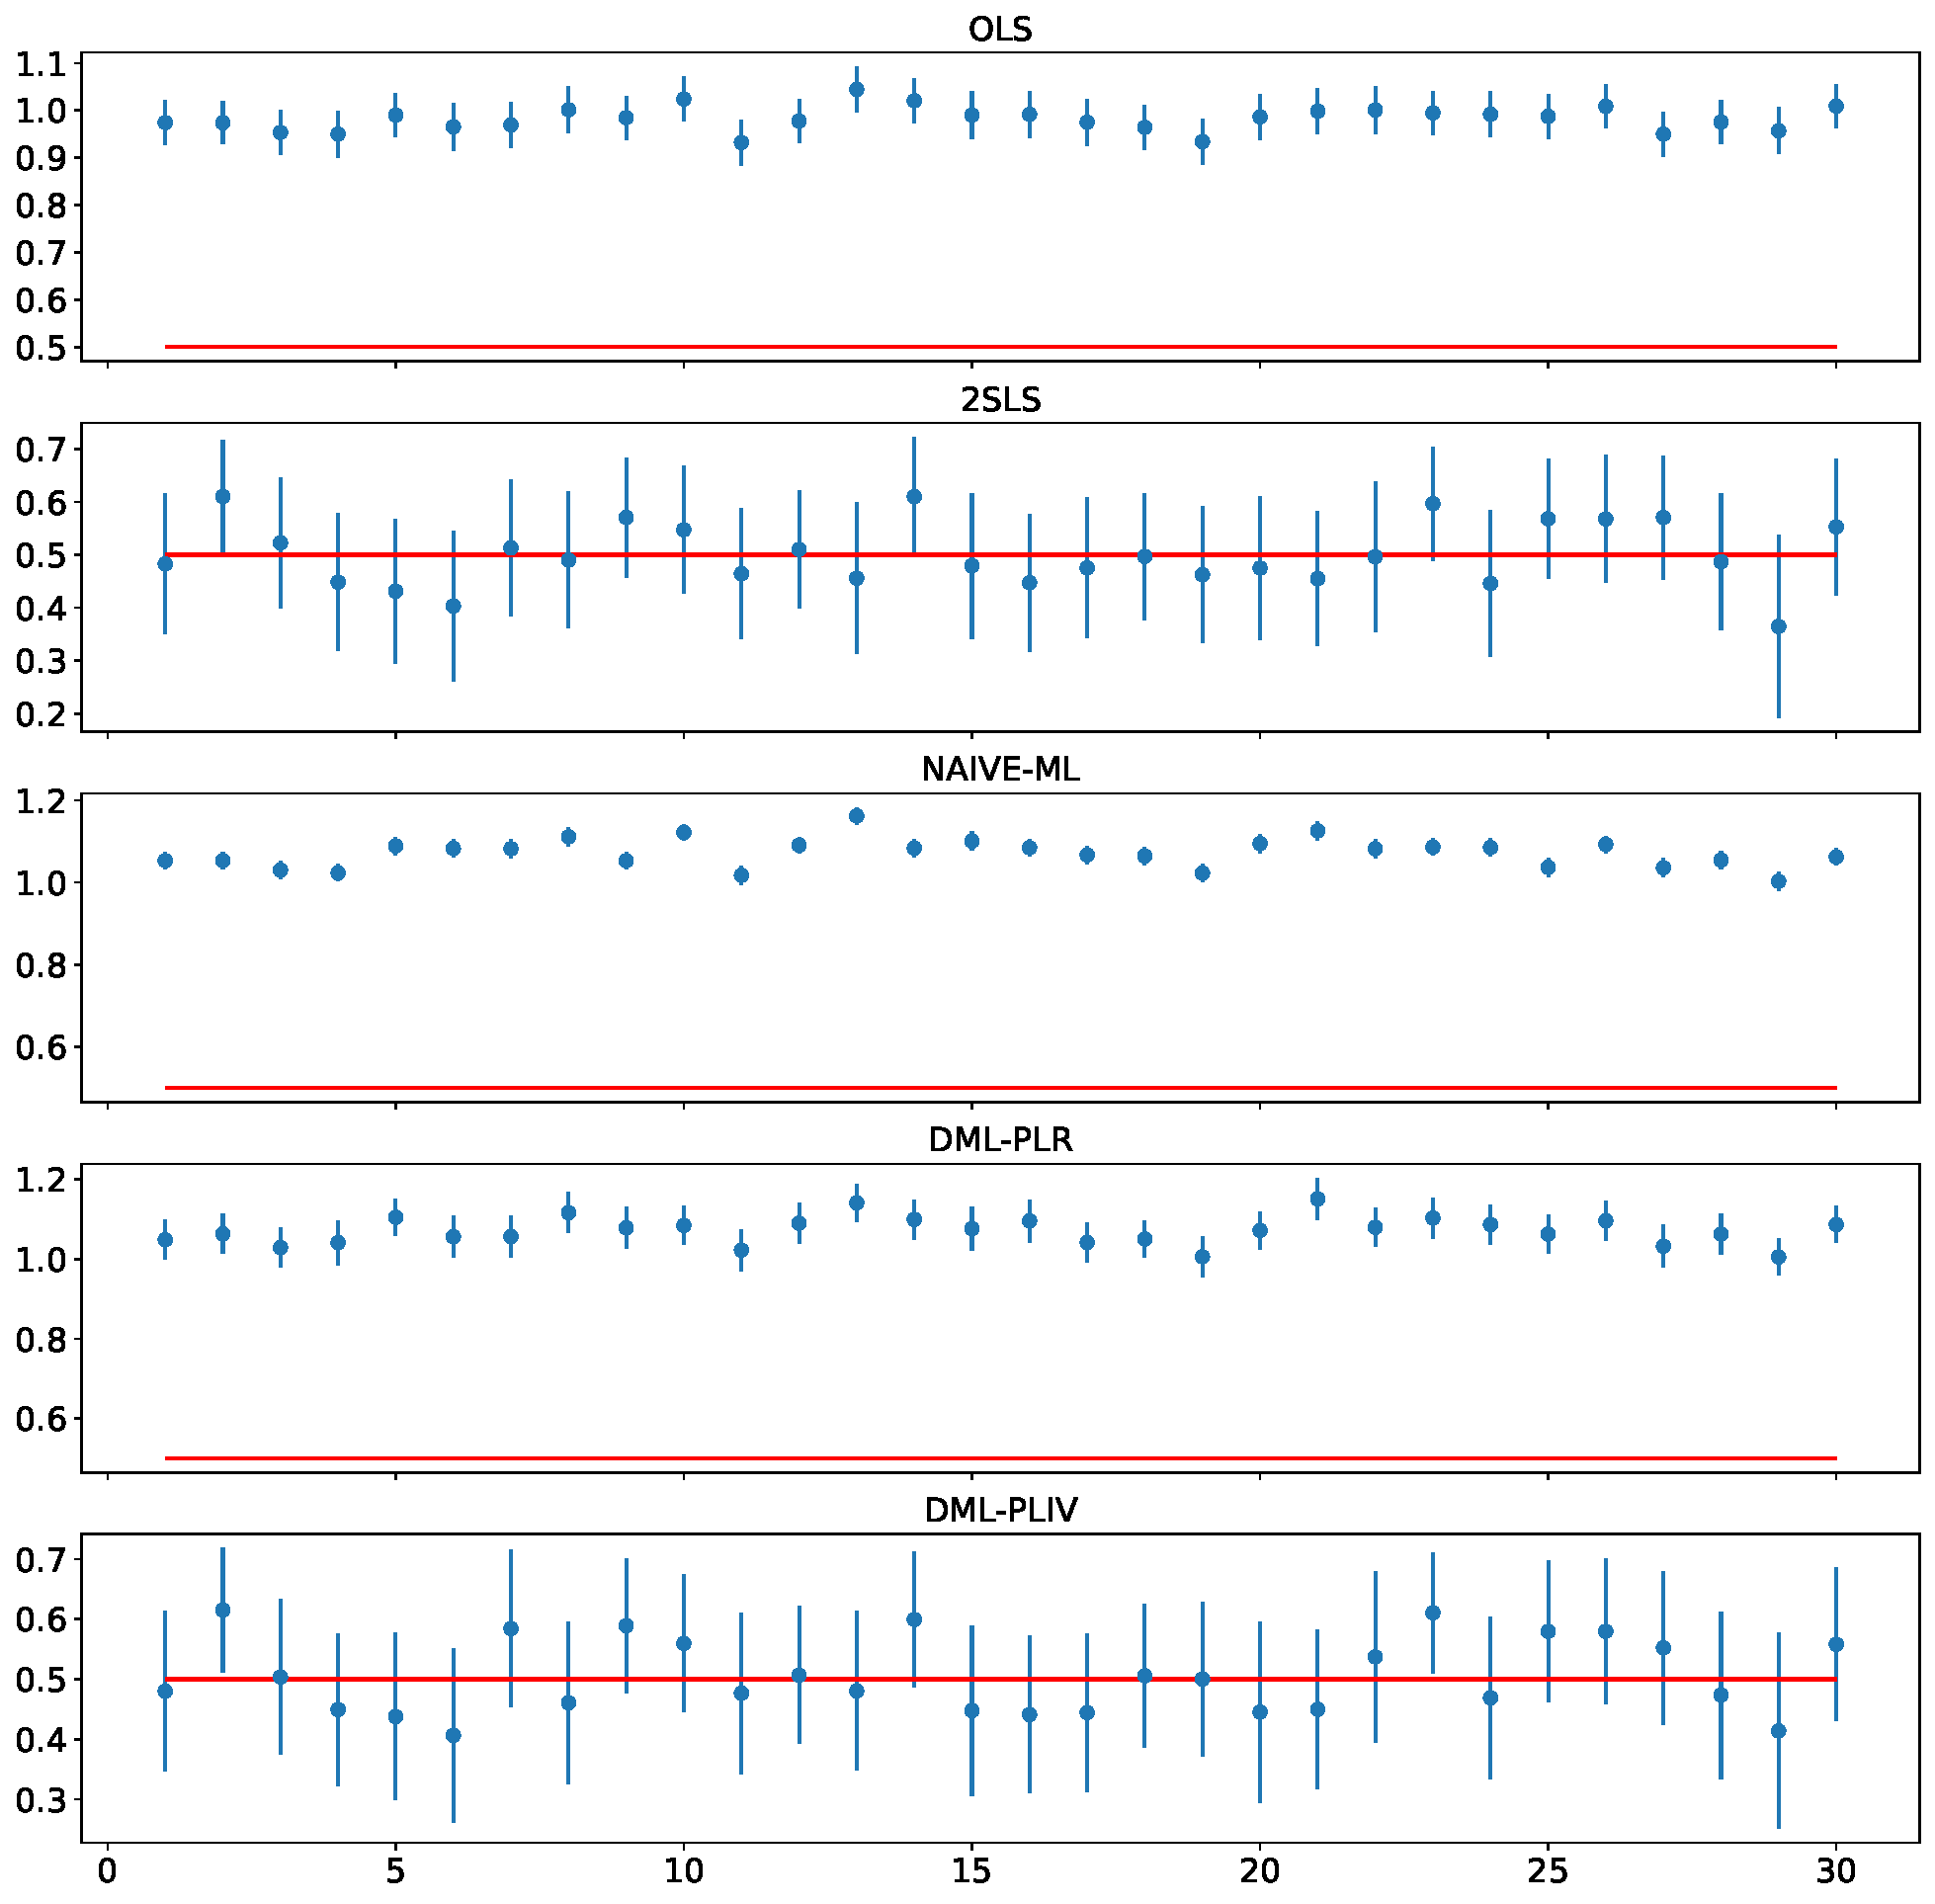
\includegraphics[width=.65\columnwidth]{\InputsPath/plots/Scenario3.pdf}
		\caption{True and estimated treatment effects per replication for Scenario 3. The error bars represent the upper and lower bound of the 95\% confidence interval of the estimate. The red line represents the true value of the treatment effect.}
		\label{Scenario3}
	\end{center}
\end{figure}
\begin{table}[H]
\centering
\caption{Scenario 3}
\label{Scenario3}
\begin{tabular}{L{3.3333333333333335cm}L{2.6666666666666665cm}R{2.0cm}R{2.6666666666666665cm}}
\toprule
{} &    RMSE &     MAE &    Bias \\
\midrule
OLS      &  0.4765 &  0.4758 &  0.4758 \\
2SLS     &  0.0783 &  0.0591 &  0.0001 \\
NAIVE-ML &  0.5788 &  0.5778 &  0.5778 \\
DML-PLR  &  0.5912 &  0.5904 &  0.5904 \\
DML-PLIV &  0.0792 &  0.0618 &   0.023 \\
Best     &    2SLS &    2SLS &    2SLS \\
\bottomrule
\end{tabular}
\end{table}

We find in Scenario 3 that the 2SLS and the DML-PLIV model tend to recover the treatment effect overall similarly in terms of how wider the confidence intervals, the RMSE, MAE and bias.  
The 2SLS model is however notable better in all three performance metrics RMSE, MAE and bias than 2SLS.

The OLS, NAIVE-ML and DML-PLR models perform worse across RMSE, MAE and bias, whereas OLS is better than the other two.

\subsection{Scenario 4}
\subsubsection{IIV model}
The Scenario 4 represents the case of a IIV model and we use the following DGP for $i=1,...,n$.
The DGP is based on the simulation experiment of \cite{Farb2020}.
\begin{eqnarray*}\label{dgp_4.1}
y_i &=& \theta d_i + x_i' \beta + u_i, \\	
d_i &=& 1\left\lbrace \alpha_x Z + v_i > 0 \right\rbrace,
\end{eqnarray*}
and
\begin{eqnarray*}\label{dgp_4.2}
\left(\begin{matrix} u_i \\ v_i \end{matrix} \right) &\sim&
\mathcal{N}\left(0, \left(\begin{matrix} 1 & 0.3 \\ 0.3 & 1 \end{matrix} \right) \right), \\
Z &\sim& \text{Bernoulli}(0.5), \\
x_i &\sim& \mathcal{N}(0, \Sigma),
\end{eqnarray*}
where $\text{Bernoulli}(p)$ represents the Bernoulli distribution with parameter $p$. 
$\Sigma$ is a matrix with entries $\Sigma_{kj} = 0.5^{|j-m|}$, with $m=1,..,k$ and $j=1,...,k$.
$\beta$ is a $(k \times 1)$ vector with entries $\beta_j=\frac{1}{j^2}$ for $j=1,...,k$ and we set $\alpha_x$ to one.
Note that the endogeneity of $D$ comes from the non-zero correlation of $u_i$ and $v_i$.
\subsubsection{Results}
\begin{figure}[H]
	\begin{center}
		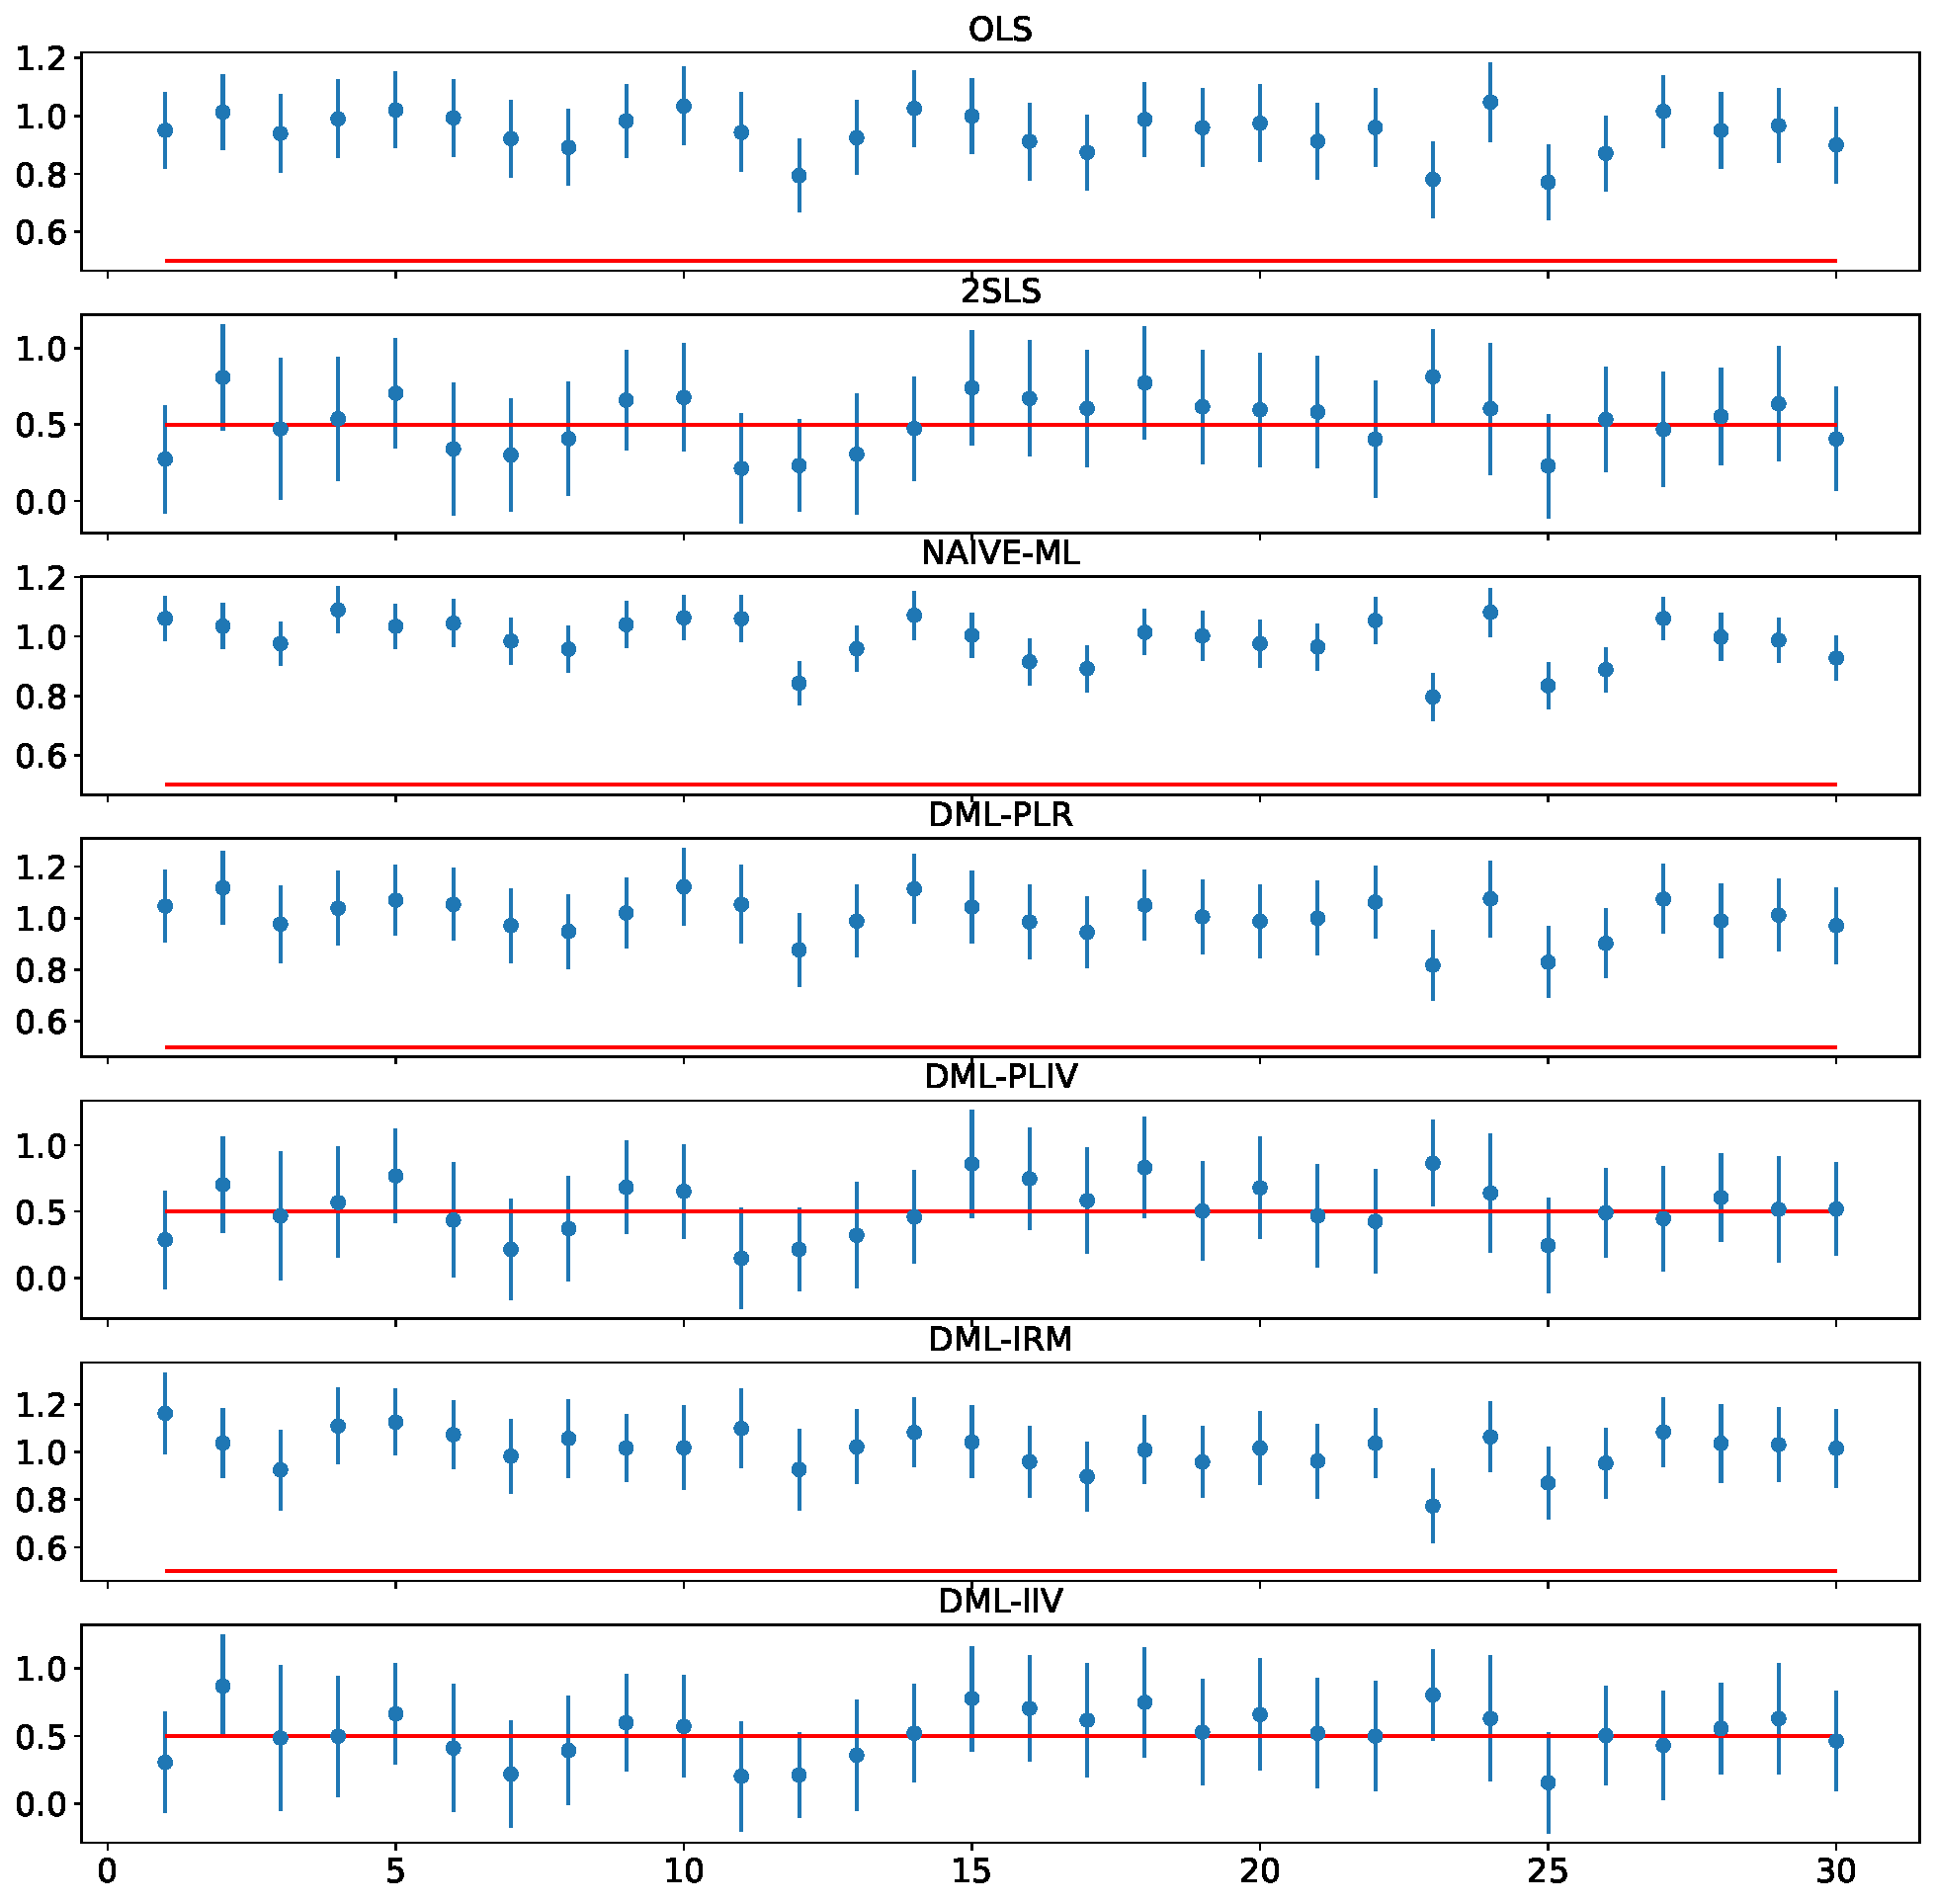
\includegraphics[width=.65\columnwidth]{\InputsPath/plots/Scenario4.pdf}
		\caption{True and estimated treatment effects per replication for Scenario 4. The error bars represent the upper and lower bound of the 95\% confidence interval of the estimate. The red line represents the true value of the treatment effect.}
		\label{Scenario 4}
	\end{center}
\end{figure}
\begin{table}[H]
\centering
\caption{Scenario 4}
\label{Scenario4}
\begin{tabular}{L{3.3333333333333335cm}L{2.6666666666666665cm}R{2.0cm}R{2.6666666666666665cm}}
\toprule
{} &    RMSE &     MAE &      Bias \\
\midrule
OLS      &   0.432 &  0.4267 &    0.4267 \\
2SLS     &  0.1846 &  0.1575 &    0.0061 \\
NAIVE-ML &  0.4499 &  0.4438 &    0.4438 \\
DML-PLR  &  0.4779 &  0.4709 &    0.4709 \\
DML-PLIV &  0.1928 &   0.165 &    0.0052 \\
DML-IRM  &  0.5139 &  0.5051 &    0.5051 \\
DML-IIV  &  0.1968 &  0.1677 &    0.0101 \\
Best     &    2SLS &    2SLS &  DML-PLIV \\
\bottomrule
\end{tabular}
\end{table}

We find in Scenario 4 that the DML-IIV, the 2SLS and the DML-PLIV model tend to recover the treatment effect overall similarly in terms of how wider the confidence intervals, the RMSE, MAE and bias.  
The DML-IIV model is however notable better in all three performance metrics RMSE, MAE and bias than the 2SLS and DML-PLIV models.

The OLS, NAIVE-ML, DML-PLR and DML-IRM models perform worse across RMSE, MAE and bias, whereas OLS is better than the other three.

\section{Conclusion}

%%%%%%%%%%%%%%%%%%%%%%%%%%%%%%%%%%%%%%%%%%%%%%%%
% Appendix:
\appendix
%\renewcommand{\thesection}{\Alph{section}}
%\setcounter{section}{0} 
\renewcommand{\thesubsection}{\Alph{subsection}}
\setcounter{subsection}{0} 
%\renewcommand{\thesubsubsection}{\Alph{subsubsection}}
%\setcounter{subsubsection}{0} 
\renewcommand{\thetable}{\Alph{table}}
\renewcommand{\thefigure}{\Alph{figure}}
\setcounter{table}{0} 
\section*{Appendix}
%\fancyhead{} % remove the header in the appendix

\begin{thebibliography}{10}
	
\bibitem{Bach2022}	
Bach, P., Chernozhukov, V., Kurz, M. S., and Spindler, M., 
\textit{DoubleML - An Object-Oriented Implementation of Double Machine Learning in Python, Journal of Machine Learning Research}, 23(53): 1-6, 
2022.

\bibitem{Bach2021}
Bach, P., Chernozhukov, V., Kurz, M. S., and Spindler, M., 
\textit{DoubleML - An Object-Oriented Implementation of Double Machine Learning in R}, 
2021.
	
\bibitem{Bell2017}
Belloni, A., Chernozhukov, V., Fernández‐Val, I. and Hansen, C., 
\textit{Program Evaluation and Causal Inference With High‐Dimensional Data}, Econometrica, 85: 233-298,
2017.

\bibitem{Cher2015}
Chernozhukov, V., Hansen, C. and Spindler, M., 
\textit{Post-Selection and Post-Regularization Inference in Linear
Models with Many Controls and Instruments},
American Economic Review: Papers and Proceedings, 105 (5): 486-90,
2015.
    
\bibitem{Cher2018}
Chernozhukov V., Chetverikov D., Demirer M., Duflo E., Hansen C., Newey W.,  Robins J.,
  \textit{Double/debiased machine learning for treatment and structural parameters},
  The Econometrics Journal, 
   21(1), pp.C1-C68,
  2018.

\bibitem{Farb2020}
Farbmacher, H., Guber, R. and Klaaßen, S.,
\textit{Instrument Validity Tests with Causal Forests}, 
MEA Discussion Paper, 13-2020,
2020.

\bibitem{frisch1933}  
  Frisch R., Waugh F.,
  \textit{Partial Time Regressions as Compared with Individual Trends}, 
  Econometrica, 1 (4), 
  387–401,
  1933. 
  
\bibitem{Lovell1963}  
  Lovell M.,
  \textit{Seasonal Adjustment of Economic Time Series and Multiple Regression Analysis},
   Journal of the American Statistical Association,
    58 (304), 
    993–1010,
    1963.
    .
\bibitem{Lovell2008}  
  Lovell M.,
   \textit{A Simple Proof of the FWL Theorem},
    Journal of Economic Education,
     39 (1), 88–91,
   	2008.
  
  
\bibitem{rob1988}
Robinson P.,  
\textit{Root-N-Consistent Semiparametric
Regression}, 
Econometrica,
 56(4):931-954,
 1988.

\end{thebibliography}


%%%%%%%%%%%%%%%%%%%%%%%%%%%%%%%%%%%%%%%%%%%%%%%%
	
\end{document}